%%%%%%%%%%%%%%%%%%%% author.tex 
%%%%%%%%%%%%%%%%%%%%%%%%%%%%%%%%%%%
%
% sample root file for your "contribution" to a proceedings volume
%
% Use this file as a template for your own input.
%
%%%%%%%%%%%%%%%% Springer 
%%%%%%%%%%%%%%%%%%%%%%%%%%%%%%%%%%


\documentclass{svproc}
%
% RECOMMENDED 
%%%%%%%%%%%%%%%%%%%%%%%%%%%%%%%%%%%%%%%%%%%%%%%%
%%%
%
\usepackage{graphicx}
\usepackage{marvosym}
\usepackage{amsmath}
\usepackage{amssymb}
\usepackage{cite}
\usepackage{color}

%\usepackage[russian]{babel}

% to typeset URLs, URIs, and DOIs
\usepackage{url}
\usepackage{hyperref}
\def\UrlFont{\rmfamily}

\def\orcidID#1{\unskip$^{[#1]}$}
\def\letter{$^{\textrm{(\Letter)}}$}

\begin{document}
\mainmatter              % start of a contribution
% Решение обратных задач химической кинетки с помощью асинхронного алгоритма глобального поиска
% Решение обратных задач химической кинетки с помощью смешанного локально-глобального поискового алгоритма 
%\title{Solving the Inverse Problems of Chemical Kinetics Using the Asynchronous Global Optimization Algorithm}
\title{Kinetic Modeling of Isobutane Alkylation with Mixed C4 Olefins and Sulfuric Acid as Catalyst Using the Asynchronous Global Optimization Algorithm}
\titlerunning{Kinetic Modeling of Isobutane Alkylation}  % abbreviated title (for running head)
%                                     also used for the TOC unless
%                                     \toctitle is used
%
\author{
Irek Gubaydullin$^{1,2}$\and
Leniza Enikeeva$^{2,3}$\orcidID{0000-0003-4219-4870}
\and
Konstantin Barkalov$^4$ \letter \orcidID{0000-0001-5273-2471}
\and
Ilya Lebedev$^4$\orcidID{0000-0002-8736-0652} 
\and
Dmitry Silenko$^4$ 
}

%
\authorrunning{I. Gubaydullin et al.} % abbreviated author list (for running head)
%
%%%% list of authors for the TOC (use if author list has to be modified)
%\tocauthor{Konstantin Barkalov and Ilya Lebedev }
%

\institute{$^1$Institute of Petrochemistry and Catalysis – Subdivision of the Ufa Federal Research Centre of RAS, Ufa, Russia\\$^2$Ufa State Petroleum Technological University, Ufa, Russia \\$^3$Novosibirsk State University, Novosibirsk, Russia\\$^4$Lobachevsky State University of Nizhny Novgorod, Nizhny Novgorod, Russia\\
\email{leniza.enikeeva@yandex.ru},
\email{konstantin.barkalov@itmm.unn.ru},
\email{ilya.lebedev@itmm.unn.ru}
}

	
\maketitle              % typeset the title of the contribution

\begin{abstract}

The paper considers the application of parallel computing technology to the simulation of catalytic chemical reaction, which is widely used in the modern automobile industry to produce gasoline with high octane number. As a chemical reaction, the process of alkylation of isobutane with mixed C4 olefins catalyzed by sulfuric acid is assumed. To simulate a chemical process, it is necessary to develop a kinetic model of the process, that is, to determine the kinetic parameters. To do this, the inverse problem of chemical kinetics is solved, which predicts the values of kinetic parameters based on laboratory data. From a mathematical point of view, the inverse problem of chemical kinetics is a global optimization problem. A parallel asynchronous information-statistical global search algorithm was used to solve it. The use of the asynchronous algorithm has significantly reduced the search time to find the optimum. The found optimal parameters of the model made it possible to adequately simulate the process of alkylation of isobutane with mixed C4 olefins catalyzed by sulfuric acid.

%обновить ключевые слова
\keywords{Global optimization $\cdot$ Multiextremal functions $\cdot$ Parallel computing $\cdot$ Chemical kinetics $\cdot$ Inverse problems }
\end{abstract}

\section{Introduction}

%Часть УГНТУ
Currently, there is a tendency to improve the environmental characteristics of automobile fuel while maintaining a high octane number. Sulfuric acid alkylation of isobutane with olefins makes it possible to obtain a high-octane component of gasoline with a minimum content of aromatic hydrocarbons. The alkylate, which is produced by the alkylation of isobutane with C3 -- C5 olefins in the presence of strong acid, has the advantages of high octane number, low vapor pressure, and zero content of olefins and aromatics that allow it to be a desirable blending component for high-quality gasoline. Alkylates will continue to act as a desirable blending component for high-quality gasoline as the quality of gasoline continues to increase \cite{cao2019}. Therefore, it is a significant process of the modern refinery. To optimize the chemical process in industry, it is necessary to first develop its model, which in this case means building a mathematical model of the chemical process and then its kinetic model, that is, numerically calculate the kinetic constants of the reaction. 


%Стыковочный абзац
As a rule, it is impossible to find out the kinetic constants of the reactions analytically. Therefore, there is a need in the development and application of numerical methods for finding the kinetic constants (see, e.g., \cite{Zaynullin2020,Enikeeva2020,Koledina2019,Enikeev2020,uskovfibrous,enikeeva2021,en13133393}). In this case, the quality criteria of the solution found (objective function) haven't an explicitt analytical description but allows an algorithmic representation and requires considerable computaton resources. Moreover, in the inverse problems of chemical kinetics the objective function can be multiextremal essentially, i.e. can have many local extrema along with the global one. 

%Часть ННГУ
The numerical methods for solving such multiextremal problems (global optimization methods) differ significantly from the local search ones (see, e.g., \cite{Sergeyev2017,PaulaviciusZilinskas2014}). As a rule, the local optimization methods cannot escape a local extremum attractione region and don't find the global optimum. At the same time, the use of the model parameters corresponding to the local solution found may appear to be insufficient since the global solution may provide a considerable advantage as compared to the local ones. 

The diversity of the global optimization problems arising entails various approaches to solving these ones. The methods of solving the global optimization problems can be divided into two classes: the metaheuristic methods and the deterministic ones. The metaheuristic algorithms, as a rule, are based on the simulation of the processes going in the nature. Some examples of the metaheuristic algorithms are simulated annealing, evolution and genetic algorithms, etc. (see e.g. \cite{Battiti2009,Eiben2015}). Because of relative simplicity, the metaheuristic algorithms are more popular among the researchers than the deterministic methods. 
However, a problem solution found by a metaheuristic algorithm is, generally speaking, a local one and may be far from the global solution \cite{Kvasov2018}. 

The possibility to construct deterministic global search methods different from the grid search and from the metaheuristic methods is related to the availability of and taking into account some {\it a priori} assumption on the properties of the problem functions. Such assumptions play a key role in the development of efficient global optimization algorithms and serve as main mathematical tools for estimating the global solutions.

An assumption on limited relative variations of the objective function values is one of natural assumptions of a problem. Such an assumption is related to the ratio of the function increment to respective increment of its argument, which is usually limited by some threshold defined by a limited energy of variations in the simulated system. In this case the functions are known as Lipschitz ones and the problem itself is called the Lipschitz global optimization problem. 

This paper presents the results of application of parallel Lipschitz optimization methods for solving the inverse problems of chemical kinetics. The main part of the paper has the following structure. The description of the mathematical model of the investigated chemical reaction is presented in Section \ref{Sec_math_mod}. The formal statement of the Lipschitz global optimization problems and the asynchronous parallel algorithm for solving these ones are described in Section \ref{Sec_GSA}. The results of the numerical solving the inverse problem of chemical kinetics are discussed in Section \ref{Sec_Exp}.

\section{Problem Statement}\label{Sec_math_mod}
%Содержательная постановка задачи

Let us consider a mathematical model of the isobutane alkylation reaction with olefins in the presence of sulfuric acid, which is a system of ordinary nonlinear differential equations (\ref{eq:one})--(\ref{eq:twelve}).

\begin{gather}
  \frac{dc_1}{dt} = -k_1c_1 + k_2c_3 - k_3c_1c_3 - k_7c_1c_2c_4 - k_{11}c_1 + k_{14}c_{11} \label{eq:one} \\
  \frac{dc_2}{dt} = -k_4c_2c_4 - k_6c_2c_5 - k_7c_1c_2c_4 - k_{15}c_{11}c_2c_4 \label{eq:two} \\
  \frac{dc_3}{dt} = k_1c_1 + k_4c_2c_5 - k_3(c_1 + c_{11})c_3 - k_{5}c_{12}c_3 - k_2c_3 + k_7c_1c_2c_4 + k_{15}c_{11}c_2c_4 \label{eq:three} \\
  \frac{dc_4}{dt} = k_3(c_1 + k_{11})c_3 - k_4c_2c_4 - k_{7}c_{1}c_2c_4 - k_{15}c_{11}c_2c_4 \label{eq:four} \\
  \frac{dc_5}{dt} = k_5c_{12}c_3 - k_{6}c_2c_5 \label{eq:five} \\
  \frac{dc_6}{dt} = k_4c_{2}c_4 \label{eq:six} \\
  \frac{dc_7}{dt} = k_6c_{2}c_5 - k_{10}c_7 \label{eq:seven} \\
  \frac{dc_8}{dt} = k_7c_{1}c_2c_4 + k_{15}c_{11}c_2c_4 + k_9c_9c_{10} - k_8c_8 \label{eq:eight} \\
  \frac{dc_9}{dt} = k_8c_{8} - k_{9}c_{9}c_{10} \label{eq:nine} \\
  \frac{dc_{10}}{dt} = k_8c_{8} - k_{9}c_{9}c_{10} \label{eq:ten} \\
  \frac{dc_{11}}{dt} = -k_3c_{11}c_3 - k_{15}c_{11}c_{2}c_4 + k_{11}c_1 + k_{12}c_{12} - k_{13}c_{11} - k_{14}c_{11} \label{eq:eleven} \\
  \frac{dc_{12}}{dt} = -k_5c_{12}c_3 + k_{13}c_{11} - k_{12}c_{12} \label{eq:twelve} 
\end{gather}

The initial conditions are $t = 0, c_1 = c_1^0; c_2=c_2^0; c_3 = 0; c_4 = 0; c_5= 0; c_6 = 0; c_7 = 0; c_8 = 0; c_9 = 0; c_{10} = 0; c_{11}=c_{11}^0; c_{12} = c_{12}^0$.
The corresponding species in eqs (\ref{eq:one})--(\ref{eq:twelve}) are 1, iC4H8; 2, iC4, 3, iC4+; 4, TMPs+; 5, DMHs+; 6, TMPs; 7, DMHs; 8, HEs; 9, iCx+; 10, iCy=; 11, 2-C4H8; 12, 1-C4H8.

As experimental data, information is taken from the article \cite{cao2019}, which represent a change in the concentrations of reaction components over time at different temperatures; as an example of experimental data at a temperature of 276.2 K, the data in Table \ref{table1} are presented.

\begin{table}
\caption{Experimental Data}
\label{table1}
\begin{center}
\begin{tabular}{ccccccc}
\hline
time, min & 1 & 2 & 5 & 10 & 15 & 20 \\
\hline\rule{0pt}{12pt}
DMH & 0.12 & 0.11 & 0.1	& 0.1 &	0.095 &	0.09  \\
TMP & 0.54 & 0.65 & 0.69 & 0.69 & 0.7 & 0.705 \\[2pt]
\hline
\end{tabular}
\end{center}
\end{table}

Thus, solving the system (\ref{eq:one})--(\ref{eq:twelve}) with the corresponding initial data, we will get a change in the calculated concentrations of the reaction components over time.

However, it is necessary to take into account the fact that the reaction rate constants $k_1, k_2, ..., k_{15}$ included in the equations (\ref{eq:one})--(\ref{eq:twelve}) are parameters depending on the reaction temperature, and this dependence is the Arrhenius equation and has the following form:

\begin{equation}
  k_i (T) = k_i^0 \exp \left(- \dfrac{E_i}{RT} \right),
  \label{eq:arren}
\end{equation}
where $k_i(T)$ is a constant of $i$-th stage of reation rate, $k_i^0$ is a pre-exponential factor of $i$-th reation stage, $E_i$ is an activation energy, J/mol, $R$ is the universal gas constant, J $\cdot$ (K$\cdot$mol), $T$ is the temperature, K. Thus, in order to fully develop the kinetic model of the reaction, it is necessary to calculate the activation energies $E_i$ and pre-exponential factors $k_i^0$ of all stages of the chemical reaction.  There are two formulations of the problems of searching for kinetic parameter data $E$ and $k^0$. The first one is to solve the inverse problem of selecting the kinetic parameters included in the equation (\ref{eq:arren}), which during the solution allow us to calculate all the reaction rate constants $k_i$. Then, with the found rate constants of the reaction stages, the system of differential equations (\ref{eq:one})--(\ref{eq:twelve}) is solved, then the calculated concentrations are compared with the corresponding experimental data. Mathematically, this problem has the following formulation: it is necessary to minimize the following objective function

\begin{equation}
  F_1 = \sum_{i=1}^I \sum_{j=1}^J \sum_{k=1}^K \left| c_{ijk}^{exp} - c_{ijk}^{calc} \right| \longrightarrow \min,
  \label{eq:objective_func1}
\end{equation}
where $c_{ijk}^{exp}$ and $c_{ijk}^{calc}$ are the experimental and calculated values of $k$-th observed component at $i$-th experiment, respectively, $I$ is the the number of observed temperatures for the reaction, ($I = 4$ in this case), $K$ is the number of experiments conducted at one temperature ($K = 3$), $M$ is the number of observed components of the reaction ($M = 2$).

The second formulation of the inverse problem of chemical kinetics implies the search for the rate constants of the stages $k_i$ included in the system (\ref{eq:one})--(\ref{eq:twelve}), separately for each temperature, then on the basis of the Arrhenius equation~(\ref{eq:arren}), the activation energies $E_i$ and the pre-exponential multipliers $k_i^0$ are calculated using the least squares method. Mathematically, this statement of the problem coincides with the equation (\ref{eq:objective_func1}), except for the first summation by temperatures:

\begin{equation}
  F_2 = \sum_{j=1}^J \sum_{k=1}^K \left| c_{ijk}^{exp} - c_{ijk}^{calc} \right| \longrightarrow \min.
  \label{eq:objective_func2} 
\end{equation}

Thus, both formulations of the problem (\ref{eq:objective_func1}) and (\ref{eq:objective_func2}) are optimization problems and the next section will describe the method that was used to solve these minimization problems.

\section{Parallel Algorithm for Solving Global Optimization Problems }\label{Sec_GSA}

\subsection{Global Optimization Problem}

\textcolor[rgb]{1,0,0}{As it has been already mentioned above, from the formal point of view we consider the inverse problem of chemical kinetics as a global optimization problem. 
In the specific problem under consideration, the values of the objective function are calculated by solving stiff ODE system (\ref{eq:one})--(\ref{eq:twelve}). Since the right parts of the system are continuous functions with bounded derivatives, then theoretically its solution will also be continuous and bounded. Therefore, the discrepancy (\ref{eq:objective_func2}) will satisfy the Lipschitz condition with a priori unknown constant.}

In the general form, a problem of the class specified above can be formulated mathematically as 
follows:
\begin{gather}
 \varphi^* = \varphi(y^\ast)=\min{\left\{\varphi(y):y\in D\right\}}, \label{problemN}\\
 D=\left\{y\in R^N: a_i\leq y_i \leq b_i, \;  1\leq i \leq N\right\} \label{D},
\end{gather}
where $a,b$ are given vectors, $a,b\in R^N$, and the objective function $\varphi(y)$ satisfies the Lipschitz condition
\begin{equation}\label{Lip}
\left|\varphi(y_1)-\varphi(y_2)\right|\leq L\left\|y_1-y_2\right\|,\; y_1,y_2 \in D.
\end{equation}

The function $\varphi(y)$ is assumed to be multiextremal and defined in the form of ``black box'' (i.e. in the form of some computing procedure, the input of which the  vector of parameters is supplied into, and the corresponding function value is taken from the output). Moreover, each \textit{trial} (i.e. the computing of the function value at a point of the search domain) is assumed to be time-consuming operation. 
As it has been noted in Introduction, such problem statement corresponds to the inverse problem of chemical kinetics completely.

The Lipschitz condition (\ref{Lip}) can be utilized to estimate the global minimum of a function within an interval, and knowing the Lipschitz constant allows constructing the global search algorithms and proving the convergence conditions for these ones (see, for example, \cite{Strongin2000}).

The growth of the computation costs with increasing problem dimensionality is one of the main difficulties in solving the multidimensional global optimization problems. The decreasing of the number of trials at preserving the solution accuracy is possible by a complete utilization of some {\it a priori} assumptions on the objective function that leads to adaptive sequential optimization algorithms.

For example, non-uniform space covering method \cite{Evtushenko2013} and simplicial partitions method \cite{Zilinskas2010} are such methods. These approaches were applied successfully for the development of the parallel optimization methods as well \cite{Evtushenko2009,Paulavicius2011}. 
Another adaptive approach to solving a multidimensional problem (\ref{problemN}) is its reduction to a single one-dimensional problem or to several ones followed by application of the one-dimensional algorithms. 
Such a reduction can be made, for example, using nested optimization scheme \cite{Grishagin2018} or Peano-Hilbert curves \cite{Barkalov2018}. 
The latter approach was used in the present work.

Using the continuous unambiguous mapping (Peano-Hilbert curve) $y(x)$ of the interval $[0,1]$ of the real axis on the hypercube $D$ from (\ref{D}), one can reduce a multidimensional problem (\ref{problemN}) to a one-dimensional problem
\[
\varphi(y^\ast)=\varphi(y(x^\ast))=\min{\left\{\varphi(y(x)): x\in[0,1]\right\}},
\]
where the function $\varphi(y(x))$ will satisfy a uniform H{\"o}lder condition
\[
\left|\varphi(y(x_1))-\varphi(y(x_2))\right|\leq H\left|x_1-x_2\right|^{1/N}
\]
with the H{\"o}lder constant $H$ linked to the Lipschitz constant $L$ by the relation $ H=2 L \sqrt{N+3}$. 
The issues of the numerical construction of various approximations of the Peano-Hilbert curve were considered in \cite{Strongin2000,Sergeyev2013}.

So far, a search trial at some point $x'\in[0,1]$ will include first the construction of the image $y'=y(x')$ and then the computing the value of the function $z'=\varphi(y')$.

%Данный комментарий можно и не включать...
%Note that the presence of rapidly decreasing components in the solution of the stiff ODE system (\ref{eq:one})--(\ref{eq:twelve}) can lead to the fact that in different subdomains the objective function can have different local Lipschitz constants. This problem will affect the convergence of any of the global optimization methods. To take it into account, a number of approaches have been proposed related to local tuning of global optimization methods (see, e.g., \cite{Barkalov2021,Strongin2020}).

\subsection{Parallel Asynchronous Global Search Algorithm}

In the approach proposed, the parallelization scheme corresponds to the ``master/worker'' principle.
In the master process the global search algorithm is executed, which accumulates the search information, evaluates the Lipschitz constant for the objective function on its base, determines the new trial points and distributes these ones among the worker processes. 

The worker processes receive the trial points from the master process, perform the new trials at these points, and send the trial results to the master process. 

Let us assume the master process to compute one point of the next trial at every iteration and to send it to a worker process for executing the trial. 
At the same time, the execution of the trial by the worker process is much more computational-costly operation than the choice of a new trial point by the master that excludes idle worker processes. 
In this case (unlike the synchronous parallel algorithms), the total number of trials executed by each worker process will depend on the computation costs of executing a particular trial and cannot be estimated in advance.

In the description of the parallel algorithm, let us assume $p+1$ computing processes to be at our disposal: one master process and $p$ worker ones.
 
At the beginning of the search, the master process (let us assume it to be Process No 0) initiates the parallel execution of $p$ trials at $p$ different points of the search domain. 
Two of these points are the boundary ones while the rest are the internal ones, i.e. at the points $\{y(x^1), y(x^2), ...,y(x^p)\}$ where 
$x^1 = 0$, $x^p = 1$, $x^i\in(0,1), i=2,..., p-1$.

Now let us assume $k\geq 0$ trials (in particular, $k$ may be equal to 0) to be completed, and the worker processes are performing the trials at the points $\{y(x^{k+1}), y(x^{k+2}), ...,y(x^{k+p})\}$. 

Each worker process having completed its trial at some point (without any loss of generality, let us assume this point to be $y(x^{k+1})$ corresponding to process No 1), sends the trial result to the master process. 
In turn, the master process selects a new trial point $x^{k+p+1}$ for the worker process according to the rules described below.
Note that in this case we will have a set of preimages of the trial points
\[
I_k = \left\{ x^{k+1},x^{k+2},...,x^{k+p} \right\},
\]
which the trials have been already started at but haven't been completed yet.

Step 1. Renumber set of preimages of the trial points 
\[
X_k = \left\{x^1, x^2,...,x^{k+p} \right\},
\]
containing all the preimages, which the trials either have been completed or are being performed at in the increasing order (by the lower index), so that
\[
0=x_1<x_2<...<x_{k+p}=1.
\]
Step 2. Compute the values 
\begin{gather*}
M_1=\max \left\{ \frac{ \left|z_i - z_{i-1} \right|}{(x_i-x_{i-1})^{1/N}} : x_{i-1} \notin I_k, x_i \notin I_k, 2\leq i\leq k+p \right\},\\
M_2=\max \left\{ \frac{ \left|z_{i+1} - z_{i-1} \right|}{(x_{i+1}-x_{i-1})^{1/N}} : x_i \in I_k, 2\leq i < k+p \right\},\\
M=\max\{M_1,M_2\},
\end{gather*}
where $z_i=\varphi(y(x_i))$ if $x_i \notin I_k, \; 1\leq i \leq k+p$. The values $z_i$ at the points $x_i \in I_k$ are undefined since the trials at the points $x_i \in I_k$ haven't been completed yet. If the value of $M$ equals 0, then set $M=1$.

Step 3. Juxtapose each interval $(x_{i-1},x_i), \; x_{i-1} \notin I_k, x_i \notin I_k, \; 2\leq i\leq k+p$ to a quantity $R(i)$, which is called a characteristic of the interval and is computed according to the formula
\begin{equation}\label{R}
R(i)=rM\Delta_i+\frac{(z_i-z_{i-1})^2}{rM\Delta_i}-2(z_i+z_{i-1}),
\end{equation}
where $\Delta_i=\left(x_i-x_{i-1}\right)^{1/N}$ and $r>1$ is the reliability parameter of the method.

Step 4. Select the interval $[x_{t-1},x_t]$, which the maximum characteristic corresponds to, i.e.
\[
R(t) = \max \left\{ R(i): \; x_{i-1} \notin I_k, x_i \notin I_k, \; 2\leq i\leq k+p \right\}.
\]

Step 5. Define the new trial point $y^{k+p+1}=y(x^{k+p+1})$, the preimage of which is $x^{k+p+1} \in (x_{t-1},x_t)$ according to the formula
\[
x^{k+p+1} = \frac{x_{t}+x_{t-1}}{2} - \mathrm{sign}(z_{t}-z_{t-1})\frac{1}{2r}\left[\frac{\left|z_{t}-z_{t-1}\right|}{M}\right]^N.
\]

Upon computing the next trial point, the master process adds it to the set $I_k$ and sends it to the worker process, which initiates the new trial at this point. 

The master process terminates the algorithm if one of two conditions is satisfied: $\Delta_{t}<\epsilon$ or $k+p>K_{max}$.
The real number $\epsilon>0$ and the integer number $K_{max}>0$ are the parameters of the algorithm and correspond to the solution search precision and to the maximum number of trials, respectively.

The parallel asynchronous algorithm described above is based on the sequential information global search algorithm. The theoretical substantiation of the algorithm convergence is given in \cite{Strongin2000}. Also, the synchronous parallelization schemes used earlier in solving a number of applied problems \cite{Kalyulin2017,Modorskii2016} are presented here.
The novelty of the present work consists in a practical implementation and application of the asynchronous parallelization scheme featured by a higher efficiency in solving the problems with different computation costs of performing the trials at different points of the search domain. 
It was confirmed by the results of experiments described in the next section.

\section{Numerical Experiments}\label{Sec_Exp}

According to the problem statements (\ref{eq:objective_func1}) and (\ref{eq:objective_func2}), the corresponding calculations were carried out in this work.
%ННГУ
To carry out the numerical experiments, UNN supercomputer Lobachevsky was used (CentOS 7.2, SLURM, two CPU Intel Sandy Bridge E5-2660 2.2 GHz and 64 Gb RAM on the node). The asynchronous global optimization algorithm was implemented using C++ (GCC 5.5.0 and Intel MPI were used); the objective function values were computed using Python 3.9.
\textcolor[rgb]{1,0,0}{The accuracy of solving the ODE system (\ref{eq:one})--(\ref{eq:twelve}) was set small enough so that the final error of the solution was much less than the accuracy of the stopping criterion of the optimization method and did not affect the method used.}

\subsection{Search for activation energies and pre-exponential multipliers of the reaction}

First, the problem of searching for activation energies and pre-exponential multipliers of all reaction stages was solved. The number of optimized parameters is 30, which is two parameters for each of the fifteen reaction stages. For activation energies, the search range was set to $0 \leq E_i \leq 100$ kJ/mol, and $0 \leq E_i \leq 10^{12}$ for pre-exponential multipliers based on physicochemical considerations. However, based on the stiffness of the system of differential equations (\ref{eq:one}) and (\ref{eq:twelve}), no solution was found in such a wide range, this is due to the too high degree of pre-exponential multipliers included in the Arrhenius equation. Therefore, during the calculations, the value of the upper bound of the pre-exponential multipliers was reduced and the solution was obtained at the upper bounds of $10^5$. The kinetic parameters found are presented in Table~\ref{table_res1}.

\begin{table}
\caption{Calculated rate constants of reaction}
\label{table_res1}
\begin{center}
\begin{tabular}{cccccccc}
\hline
 & $k_1$ & $k_2$ & $k_3$ & $k_4$ & $k_5$ & $k_6$ & $k_7$\\
\hline\rule{0pt}{12pt}
$E$, kJ / mol & 98.60 & 98.22 & 99.07 & 2.29 & 97.61 & 94.30 & 8.67\\
$k^0$ & $1.46\cdot10^3$ & $1.53\cdot10^2$ & $1.03\cdot10^4$ & $1.10$ & $4.99\cdot10^2$  & $1.31\cdot10^2$ & $5.45\cdot10^2$\\
\hline
$k_8$ & $k_9$ & $k_{10}$ & $k_{11}$ & $k_{12}$ & $k_{13}$ & $k_{14}$ & $k_{15}$ \\
\hline\rule{0pt}{12pt}
11.57 & 73.16 & 65.54 & 13.86 & 4.93 & 2.69 & 21.19 & 0.63\\
$2.60\cdot10^2$ & $3.95\cdot10^4$ & $3.24\cdot10^4$ & $1.73\cdot10$ & $3.43$ & $1.78$ & $1.42\cdot10^3$ & $5.57\cdot10$\\[2pt]
\hline
\end{tabular}\end{center}\end{table}

%ННГУ
To evaluate the efficiency of the implemented optimization method, the results obtained using the sequential algorithm, the parallel synchronous, and the parallel asynchronous ones with the use of 8 nodes when solving the problem in the above statement were compared.  
The minimum values of the objective function found by respective methods, the times of solving the problem (in hours), and the values of speedup in time are presented in Table \ref{table_30D}. 
During the experiments the parameter of the method $r=3.0$ from (\ref{R}) and the accuracy  $\epsilon = 10^{-3}\left\|b-a\right\|$ in the termination condition were used. Once the global search method achieves the preset accuracy, the solution was refined by Hook-Jeeves local method \cite{HookJeeves} with the accuracy $\epsilon = 10^{-5}\left\|b-a\right\|$.

\begin{table}
\caption{Indicators achieved when solving the problem with 30 parameters}
\label{table_30D}
\begin{center}
\begin{tabular}{cccc}
\hline\noalign{\smallskip}
 Method      & Minimum  & Time (h.) & Speedup \\
\hline\noalign{\smallskip}
Serial       & 7.6   &    3.8     &  ---        \\
Synchronous  & 5.9   &   0.9     &   4.3       \\
Asynchronous & 4.8   &   1.1     &   3.6       \\
\noalign{\smallskip}\hline
\end{tabular}\end{center}\end{table}

The results have shown that both parallel algorithms had demonstrated a moderate speedup but had found better solutions than the sequential method. At that, the asynchronous algorithm had found a better solution than synchronous one. This explains also a smaller speedup of the asynchronous algorithm as compared with the synchronous one since the asynchronous method had executed more trials in the course of search for the optimal kinetic parameters of the problem.

%Часть УГНТУ
With the help of the obtained kinetic parameters, the direct problem of chemical kinetics was solved. However, the calculated kinetic curves poorly described the experimental data, which is confirmed by Fig. \ref{fig:res1}. It can be seen that the character of the calculated curve does not match the experimental dependence.

\begin{figure}
\begin{center}
  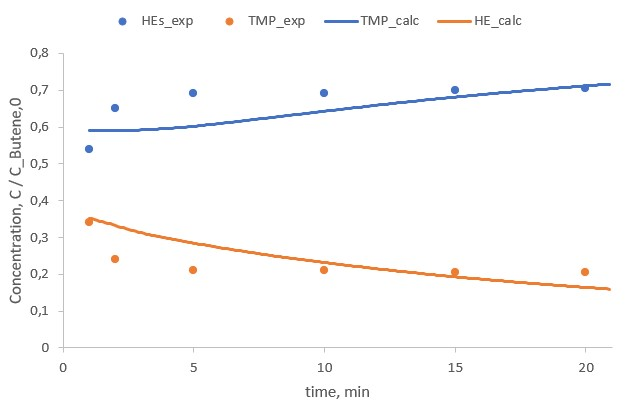
\includegraphics[width=0.7\linewidth]{res1.jpg}
  \caption{Concentration profiles of key components when calculating the activation energies and pre-exponential reaction multipliers according to the problem statement~\ref{eq:objective_func1}. Temperature: 276.2 K. Symbols, experimental data; line, calculated values.}
  \label{fig:res1}  
\end{center}
\end{figure}

Therefore, it was decided to carry out calculations according to the second formulation of the problem (\ref{eq:objective_func2}), namely, to calculate the constants of each reaction stage separately, then, according to the Arrhenius dependence, find the kinetic parameters $E_i$ and $k_i^0$.

\subsection{Searching for rate constants separately for each temperature}

Next, the problem of finding constants $k_i$ of the reaction stages included in the system (\ref{eq:one})--(\ref{eq:twelve}) was solved. Velocity constants were calculated for each of the temperatures (Table \ref{table_res2}).

\begin{table}[ht]
\caption{Calculated rate constants}\label{table_res2}
\begin{center}
\begin{tabular}{cccccccc}
\hline
T, K & $k_1$ & $k_2$ & $k_3$ & $k_4$ & $k_5$ & $k_6$ & $k_7$\\
\hline\rule{0pt}{12pt}
276.2 & 1.66 & 0.13 & 2.09 & 0.08 & 0.11 & 1.83 & 8.82 \\
279.2 & 1.94 & 0.33 & 2.19 & 0.32 & 0.16 & 1.96 & 14.15\\
282.2 & 2.14 & 0.99 & 5.43 & 2.77 & 0.56 & 2.13 & 45.85\\
286.2 & 2.43 & 0.99 & 5.51 & 2.81 & 0.56  & 2.35 & 58.97\\
\hline
$k_8$ & $k_9$ & $k_{10}$ & $k_{11}$ & $k_{12}$ & $k_{13}$ & $k_{14}$ & $k_{15}$ \\
\hline\rule{0pt}{12pt}
0.87 & 13.38 & 13.71 & 12.57 & 4.20 & 18.54 & 2.70 & 58.61\\
1.05 & 13.39 & 14.50 & 24.26 & 7.67 & 19.41 & 3.86 & 74.64\\
1.09 & 18.92 & 17.41 & 33.73 & 6.07 & 19.24 & 9.61 & 77.37\\
1.50 & 24.09 & 17.88 & 34.22 & 4.35 & 23.04 & 16.38 & 94.45\\[2pt]
\hline
\end{tabular}\end{center}\end{table}

%ННГУ
When solving this problem, the operation performances of the sequential algorithm, of the parallel synchronous, and of the parallel asynchronous ones were also compared.  
The minimum values of the objective function found by respective methods, the time of solving the problem (in hours), and the speedup in time with the use of 8 nodes are presented in Table \ref{table_15D}. All the parameters of the method were the same as in the previous run. 

\begin{table}
\caption{Indicators achieved when solving the problem with 15 parameters}
\label{table_15D}
\begin{center}
\begin{tabular}{cccc}
\hline\noalign{\smallskip}
 Method      & Minimum  & Time (h.) & Speedup \\
\hline\noalign{\smallskip}
Serial       & 0.35   &   3.4     &  ---        \\
Synchronous  & 0.36   &   0.4     &   8.6       \\
Asynchronous & 0.35   &   0.2     &   16.6       \\
\noalign{\smallskip}\hline
\end{tabular}\end{center}\end{table}

The results have shown that all algorithms had found good solutions (in the values of the objective function). At that, the asynchronous algorithm had demonstrated two times higher speedup than the synchronous one. A good speedup of the asynchronous algorithm remains at a greater number of nodes as well, the results of its work are presented in Table \ref{tab_parall}.

\textcolor[rgb]{1,0,0}{Note that when solving the global optimization problem, the number of iterations of the parallel algorithm (and hence its speedup) depends significantly on the estimation of the Lipschitz constant of the objective function. The constant is adaptively estimated during the work of the algorithm and may vary depending on the accumulated search information. With a correct estimate of the Lipschitz constant the method can converge to a global optimum point faster than in the case of its incorrect estimate. This explains the effect of superlinear speedup observed in experiments.}

\begin{table}
\caption{Speedup of the asynchronous parallel algorithm}
\label{tab_parall}
\begin{center}
\begin{tabular}{cccc}
\hline\noalign{\smallskip}
Nodes  & Minimum  & Time (h.) & Speedup \\
\hline\noalign{\smallskip}
1  & 0.35   &   3.4     &   ---        \\
8  & 0.35   &   0.2     &   16.6       \\
16 & 0.36   &   0.1     &   34.3       \\
32 & 0.35   &   0.06    &   59.5       \\
\noalign{\smallskip}\hline
\end{tabular}\end{center}\end{table}

%Часть УГНТУ
The direct problem of chemical kinetics was solved with the found rate constants, the results of comparison with experimental data are shown in Fig. \ref{fig:res2} (an experiment at a temperature of 276.2 K is presented). We see that this time the description of the data turned out to be rather accurate.

\begin{figure}
\begin{center}
  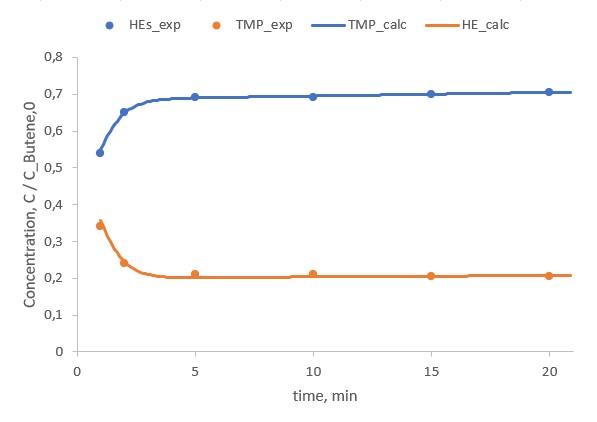
\includegraphics[width=0.7\linewidth]{res2.jpg}
  \caption{Concentration profiles of key components when calculating the rate constants according to the problem statement~\ref{eq:objective_func2}. Temperature: 276.2 K. Symbols, experimental data; line, calculated values.}
  \label{fig:res2}  
\end{center}
\end{figure}

After calculating the rate constants for different temperature values, it is possible to calculate the parameters $E_i$ and $k_i^0$. So, for example, for the first stage of the reaction $E_1 = 24.65$ kJ/mol, $k_1^0 = 6.85 \cdot 10^4$ min$^{-1}$, for the third stage $E_3 = 75.57$ kJ/mol, $k_3^0 = 2.62 \cdot 10^{14}$ kg $\cdot$mol$^{-1}\cdot$min$^{-1}$. However, for some stages, the parameter values were fairly high $k^0$, namely for the second stage $k_2^0 = 8.52 \cdot 10^{25}$ min$^{-1}$, for the seventh stage $k_7^0 = 2.82 \cdot 10^{26}$ kg mol$^{-2}$ min$^{-2}$. Therefore, in future works, the constants corresponding to these kinetic parameters will be recalculated.

\section{Conclusions and Future Work}
Thus, the article describes the search for kinetic parameters of the industrial chemical reaction of isobutane alkylation with olefins in the presence of sulfuric acid. A search was made for the rate constants of all reaction stages, as well as activation energies and pre-exponential multipliers have been calculated. The optimization method allowed us to find a fairly accurate description of the experimental data. In the future, it is planned to use this method and parallelization to eliminate high values of the pre-exponential reaction multipliers and to search for optimal conditions for the alkylation reaction using the developed kinetic model.

\medskip

\textbf{Acknowledgments}. This study was supported by the Russian Science Foundation, project No.\,21-11-00204, and by RFBR, project No.\,19-37-60014.

%
% ---- Bibliography ----
%
\bibliographystyle{spmpsci}
\bibliography{bibliography}{}

\end{document}
